% Figure from MATH 591 notes, section 60. Compile with the notes preamble.
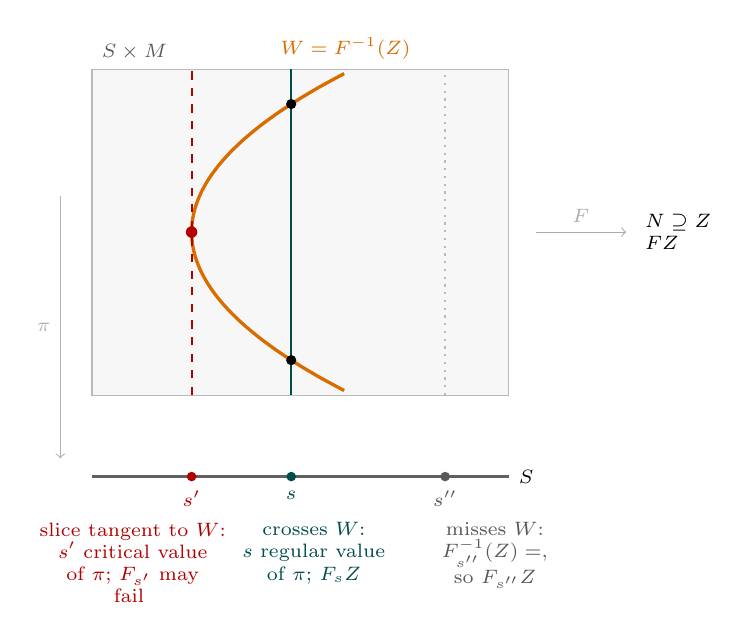
\begin{tikzpicture}[scale=1.15, font=\scriptsize]
\fill[gray!6] (0,0) rectangle (4.6,3.6); \draw[gray!55] (0,0) rectangle (4.6,3.6);
\node[gray!70!black, anchor=south west] at (0,3.6) {$S \times M$};
% W = F^{-1}(Z): sideways parabola s = s' + c (m - 1.8)^2
\draw[orange!85!black, very thick] plot[smooth, domain=-1.75:1.75] ({1.1+0.55*\x*\x},{1.8+\x});
\node[orange!85!black, anchor=south] at (2.8,3.6) {$W = F^{-1}(Z)$};
% slices
\draw[red!70!black, dashed, thick] (1.1,0) -- (1.1,3.6);
\draw[teal!60!black, thick] (2.2,0) -- (2.2,3.6);
\draw[gray!55, dotted, thick] (3.9,0) -- (3.9,3.6);
\fill[red!70!black] (1.1,1.8) circle (1.8pt);
\fill (2.2,{1.8+sqrt(1.1/0.55)}) circle (1.6pt); \fill (2.2,{1.8-sqrt(1.1/0.55)}) circle (1.6pt);
% parameter line S
\draw[thick, gray!75!black] (0,-0.9) -- (4.6,-0.9) node[right, text=black] {$S$};
\draw[->, gray!60] (-0.35,2.2) -- node[left] {$\pi$} (-0.35,-0.7);
\foreach \x/\c/\l in {1.1/red!70!black/{s'},2.2/teal!60!black/s,3.9/gray!70!black/{s''}} {\fill[\c] (\x,-0.9) circle (1.5pt); \node[\c, below] at (\x,-0.95) {$\l$};}
% outcomes
\node[red!70!black, align=center, anchor=north] at (0.45,-1.3) {slice tangent to $W$:\\ $s'$ critical value\\ of $\pi$; $F_{s'}$ may\\ fail $\pitchfork$};
\node[teal!60!black, align=center, anchor=north] at (2.45,-1.3) {crosses $W$:\\ $s$ regular value\\ of $\pi$; $F_s \pitchfork Z$};
\node[gray!70!black, align=center, anchor=north] at (4.45,-1.3) {misses $W$:\\ $F_{s''}^{-1}(Z) = \varnothing$,\\ so $F_{s''} \pitchfork Z$};
% the map F
\draw[->, gray!65] (4.9,1.8) -- node[above] {$F$} (5.9,1.8);
\node[anchor=west, align=left] at (6.0,1.8) {$N \supseteq Z$\\ $F \pitchfork Z$};
\end{tikzpicture}
